\subsection{SELECTORATE THEORY}
The selectorate theory represents one version of the strategic perspective.

In selectorate theory, leaders build a coalition of supporters among the selectorate. The selectorate (S) consists of those who have at least a nominal say in choosing leaders and are eligible to become members of a winning coalition. The winning coalition (W) is the subset of the selectorate without whose support an incumbent cannot be sustained in office.

\textbf{Leaders attempt to retain the loyalty of their supporters by giving them more benefits than any domestic political opponent can credibly promise to deliver.}
Rewards come in two varieties:


\begin{enumerate}
    \item [(1)] private goods:
    \item [] Private goods are rewards that benefit only those who get them—that is, members of the leader’s essential coalition of supporters.
    \item [] Examples might include privileged access to government contracts, exploitation of a black market, or protection against prosecution.
    \item [(2)] public goods.
    \item [] Public goods are government policies and programs that all people benefit from whether they are in the leader’s inner circle or not.
    \item [] Examples of public goods include national defense, free speech and free assembly, public parks, equal protection under the law, and free access to education.
\end{enumerate}

The selectorate theory's five rules of governance are as follows:

\begin{enumerate}
    \item Depend on as few key people to keep you in power as possible.
    
    \item Draw that small group of essential coalition members from as large a pool of people as possible.
    
    \item Tax people as much as possible, subject to the constraints that they continue to work and pay taxes rather than take siestas, and that they are not made so miserable that they decide it is worthwhile to risk revolting rather than continue to live with the existing political system.
    
    \item Reward your essential backers just enough so they stick with you rather than shopping around for a new leader who might do more for them.
    
    \item Don't spend resources on benefiting the general population when those resources are needed to keep the loyalty of the members of your essential coalition.
\end{enumerate}

\begin{center}
    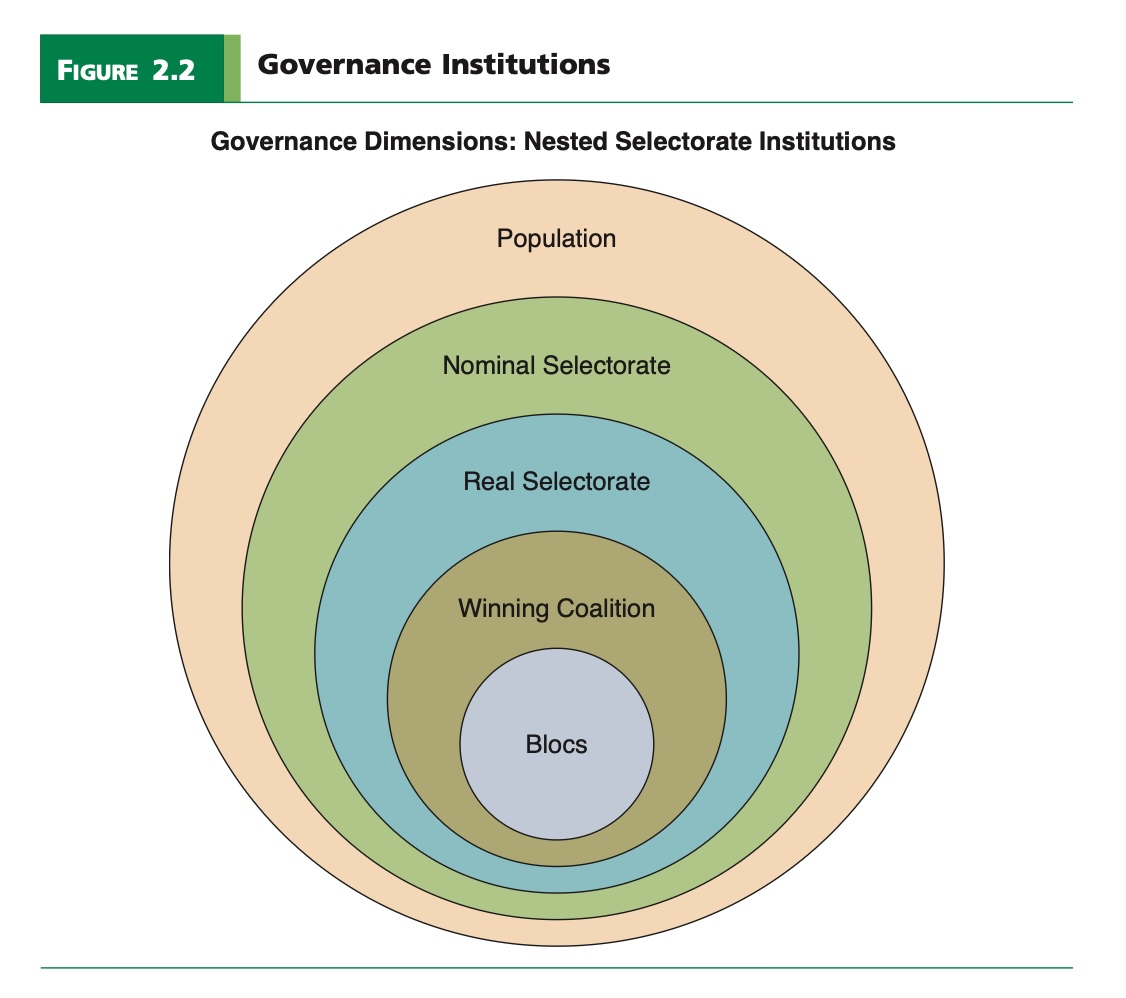
\includegraphics[width=0.7\textwidth]{images/nested_selectorate_institutions.jpg}
    \captionof{figure}{\label{fig:fig3_nested_selectorate_institutions}%\textit{\parencite[Fig.\(\backsim\)1]{cranmerWhatCanWe2017}}
    }
\end{center}

When domestic institutions constrain a leader to require a broad base of support private rewards are an inefficient way to retain power (de Tocqueville 2000; Lake and Baum 2001; Bueno de Mesquita et al. 2003; Bueno de Mesquita and Smith 2011). Democratic leaders would have to spread these rewards across so many people that each would receive too little for the benefits to influence their loyalty to the incumbent.

When political institutions compel a leader to depend on many supporters so that a bundle of public goods is the reward for retaining the incumbent, \textbf{the institutions of governance induce weak loyalty to the incumbent}.

